% Milestone 2 slides. Build: tectonic reports/milestone2/slides.tex
\documentclass[aspectratio=169,10pt]{beamer}
\usetheme[progressbar=frametitle,numbering=fraction]{metropolis}
\usepackage{polyglossia}
\setmainlanguage{polish}
\usepackage{booktabs}
\usepackage{graphicx}

% Same hues as the EDA figures: ham = blue, spam = orange.
\definecolor{ham}{HTML}{2A78D6}
\definecolor{spam}{HTML}{EB6834}
\definecolor{spamtext}{HTML}{B4451A}
\definecolor{ink}{HTML}{1B1F24}
\setbeamercolor{frametitle}{bg=ink}
\setbeamercolor{progress bar}{fg=spam,bg=ink!20}
\setbeamercolor{title separator}{fg=spam}
\setbeamercolor{alerted text}{fg=spamtext}
\setbeamercolor{block title}{bg=ink!10,fg=ink}
\setbeamercolor{block body}{bg=ink!4}

\newcommand{\ham}{\textcolor{ham}{\textbf{ham}}}
\newcommand{\spam}{\textcolor{spamtext}{\textbf{spam}}}

\title{Wykrywanie spamu w wiadomościach SMS}
\subtitle{Milestone 2}
\author{Jerzy Czarnecki \and Mateusz Małachowski \and Sebastian Rydz \and Wojciech Wójcik}
\date{12.11.2026}

\begin{document}


\maketitle

\begin{frame}{B0, reguła B0r i B1: punkty odniesienia}
  \begin{columns}[T]
    \begin{column}{0.5\textwidth}
      \begin{itemize}
        \item Zamrożony podział z M1: te same 837 rekordy testowe dla wszystkich wariantów
        \item \textbf{B0}: zawsze \ham{}, F1 spamu = 0
        \item \textbf{B0r}: spam, gdy jest $\geq$ 1 znacznik z EDA (telefon, kwota, kod krótki, URL); próg $k$ z walidacji
        \item \textbf{B1}: surowy tekst $\to$ TF-IDF $\to$ regresja logistyczna
        \begin{itemize}
          \item małe litery, domyślny \texttt{token\_pattern}, unigramy, L2
          \item TF-IDF tylko na treningu; \texttt{C} = 300 i próg z walidacji
        \end{itemize}
      \end{itemize}
    \end{column}
    \begin{column}{0.46\textwidth}
      \centering\small
      \begin{tabular}{lrrr}
        \toprule
        test & B0 & B0r & B1 \\
        \midrule
        F1 spam        & 0,000 & 0,936 & \textbf{0,940} \\
        precision spam & 0,000 & 0,963 & 0,990 \\
        recall spam    & 0,000 & 0,912 & 0,894 \\
        PR-AUC         & 0,135 & 0,915 & 0,980 \\
        FP / FN        & 0 / 113 & 4 / 10 & 1 / 12 \\
        \midrule
        F1 spam (val)  & 0,000 & 0,905 & 0,922 \\
        \bottomrule
      \end{tabular}\\[0.6em]
      {\small B1 $-$ B0r na teście: +0,3 p.p., CI [$-$3,6; +4,2]. Reguła łapie większość spamu, B1 daje mniej fałszywych alarmów i lepszy ranking.}
    \end{column}
  \end{columns}
\end{frame}

\begin{frame}{P1--P3: ten sam wektoryzator, to samo \texttt{C}, inny tekst}
  \small
  \centering
  \begin{tabular}{llrrrr}
    \toprule
    & & \multicolumn{2}{c}{walidacja} & \multicolumn{2}{c}{test} \\
    \cmidrule(lr){3-4}\cmidrule(lr){5-6}
    wariant & zmiana tekstu & F1 spam & PR-AUC & F1 spam & FP / FN \\
    \midrule
    B1  & brak                                  & 0,922 & 0,962 & 0,940 & 1 / 12 \\
    P1  & \texttt{\_phone\_ \_shortcode\_ \_money\_} & \textbf{0,959} & 0,974 & \textbf{0,959} & 1 / 8 \\
    P2a & URL $\to$ \texttt{\_url\_}             & 0,926 & 0,963 & 0,944 & 1 / 11 \\
    P2b & URL usunięty                          & 0,906 & 0,957 & 0,919 & 1 / 16 \\
    P3  & \texttt{sooo}$\to$\texttt{soo}, \texttt{!!!}$\to$\texttt{!!} & 0,922 & 0,963 & 0,940 & 1 / 12 \\
    \midrule
    \multicolumn{2}{l}{\textbf{P2a+P1+P3} (wybrany na walidacji)} & 0,968 & 0,975 & 0,954 & 0 / 10 \\
    \bottomrule
  \end{tabular}\\[1em]
  \raggedright
  \begin{itemize}
    \item Próg decyzji osobno dla każdego wariantu, tylko na walidacji. Wariant końcowy wybrany na walidacji, test tylko raportujemy.
    \item Łączymy warianty, które na walidacji nie pogorszyły F1 ani PR-AUC. P3 w połączeniu nic nie zmienia (remis z P2a+P1).
  \end{itemize}
\end{frame}

\begin{frame}{Czy poprawa jest pewna? Bootstrap sparowany na teście}
  \begin{columns}[T]
    \begin{column}{0.56\textwidth}
      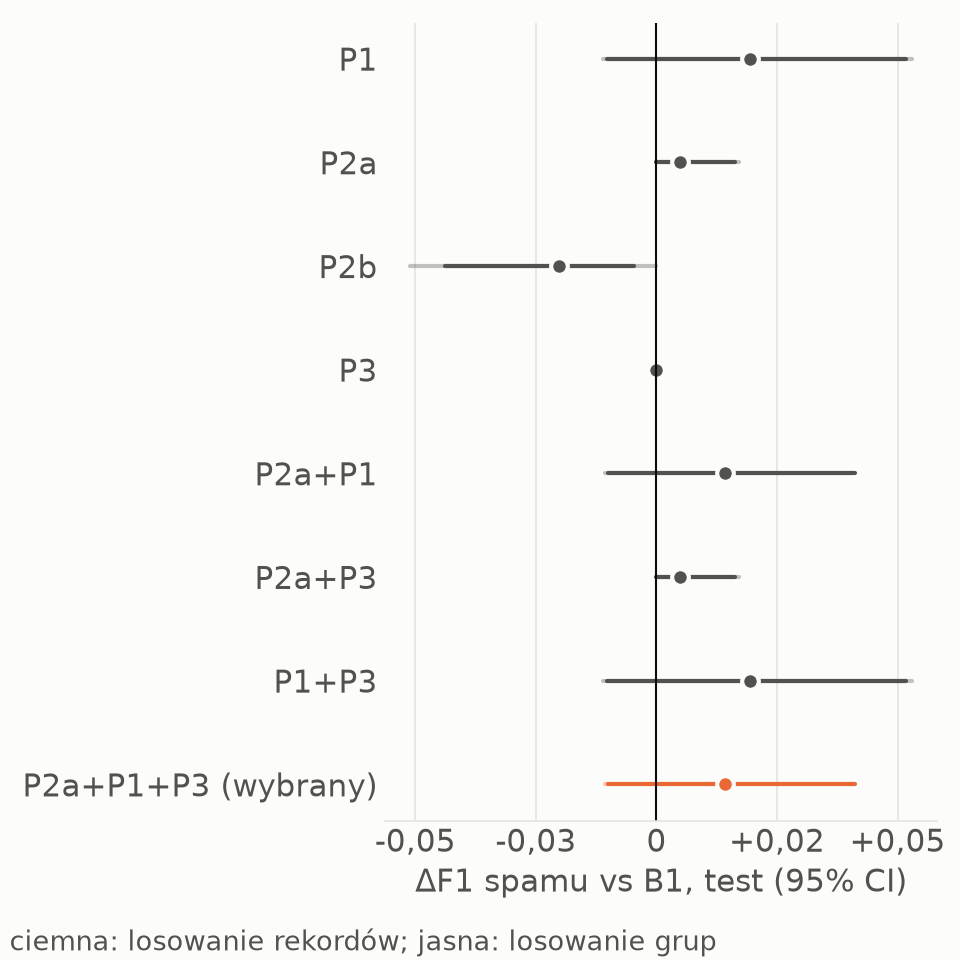
\includegraphics[width=\linewidth,height=0.8\textheight,keepaspectratio]{fig_delta.png}
    \end{column}
    \begin{column}{0.42\textwidth}
      \small
      \begin{itemize}
        \item \textbf{P1}: +1,9 p.p., CI [$-$1,0; +5,2]. Kierunek zgodny z H1, ale 113 spamów to za mało na pewność.
        \item \textbf{P2b}: $-$2,0 p.p., CI [$-$4,4; $-$0,5]. Usuwanie URL szkodzi, bo model korzysta z domen (H2).
        \item \textbf{P3}: identyczne predykcje jak B1 na czystym tekście (H3).
        \item Wybrany wariant: +1,4 p.p., CI [$-$1,0; +4,1].
        \item Losowanie całych grup duplikatów daje podobne lub nieco szersze przedziały.
      \end{itemize}
    \end{column}
  \end{columns}
\end{frame}

\begin{frame}{Trudniejsze warunki: podzbiory testu i literówki}
  \begin{columns}[T]
    \begin{column}{0.5\textwidth}
      \textbf{F1 spamu na podzbiorach testu}\\[0.4em]
      \small
      \begin{tabular}{lrrr}
        \toprule
        podzbiór & spam & B1 & wybrany \\
        \midrule
        cały test           & 113 & 0,940 & 0,954 \\
        bez duplikatów      & 102 & 0,938 & 0,954 \\
        podobieństwo $<$ 0,5 &  72 & 0,902 & 0,925 \\
        \bottomrule
      \end{tabular}\\[0.6em]
      Bez kampanii podobnych do treningu oba modele tracą 3--4 p.p.
    \end{column}
    \begin{column}{0.46\textwidth}
      \textbf{Literówki w X\% słów testu} {\small (3 ziarna)}\\[0.4em]
      \small
      \begin{tabular}{lrrr}
        \toprule
        & 0\% & 10\% & 20\% \\
        \midrule
        B1       & 0,940 & 0,936 & 0,917 \\
        P3       & 0,940 & 0,936 & 0,922 \\
        wybrany  & 0,954 & 0,949 & 0,947 \\
        \bottomrule
      \end{tabular}\\[0.6em]
      Odchylenie między ziarnami $\approx$ 0,01, więc zysk P3 mieści się w szumie. Maski numerów nie zależą od pisowni.
    \end{column}
  \end{columns}
\end{frame}

\begin{frame}{Problemy i plan na Milestone 3}
  \begin{columns}[T]
    \begin{column}{0.48\textwidth}
      \textbf{Problemy}
      \begin{itemize}
        \item Różnice między wariantami to kilka SMS-ów: 1 spam $\approx$ 0,9 p.p.\ recall.
        \item Prosta reguła jest blisko B1, więc znaczniki niosą większość sygnału; P1 przenosi je do modelu.
        \item Na teście sam P1 wypada lepiej niż wybrane połączenie. Nie zmieniamy wyboru, bo byłby to dobór na teście.
        \item Niewykryte spamy to głównie wiadomości bez numeru i URL (randki, reklamy) albo z numerem w dziwnej formie (\texttt{146tf150p}).
      \end{itemize}
    \end{column}
    \begin{column}{0.48\textwidth}
      \textbf{Plan M3}
      \begin{itemize}
        \item Stabilność efektu P1: powtórzona grupowa walidacja krzyżowa na train+val
        \item P4: dekodowanie encji HTML (\texttt{\&lt;\#\&gt;}) jako analiza wrażliwości
        \item Osobny eksperyment: n-gramy słowne vs znakowe
        \item Model M: zamrożone embeddingi zdań + regresja logistyczna, strojenie na walidacji
      \end{itemize}
    \end{column}
  \end{columns}
\end{frame}

\end{document}
